% Greenhill & Subrahmanyan

%\setcounter{chapter}{6} 

\chapter{Global Signal Instrumentation}

\begin{bf}
\author{  
L. J. Greenhill 
(Harvard-Smithsonian Center for Astrophysics) \\
R. Subrahmanyan 
(Raman Research Institute)   
}\\

\noindent
Experiments that seek to detect a global (zero-mode) HI signature during the Epoch of Reionization and Cosmic Dawn use purpose-built meter-wave instrumentation.  For the EOR, radiometry has contributed early constraints on models.   For Cosmic Dawn, the EDGES, SARAS, and LEDA efforts are active.  Radiometry by EDGES has delivered a first claim of detection but independent confirmation is not yet in hand. This chapter presents the rudiments of radiometry instrumentation, discussion of concepts that bear on design, and challenges going forward. \\

\end{bf}

\section{Introduction}

Two experiments have established limits on the predicted sky-averaged (zero-mode) signature from HI emission at redshifts ($z$) associated with the Epoch of Reioniation (EOR).  The {\underline E}xperiment to {\underline D}etect the {\underline G}lobal {\underline E}OR {\underline S}ignature -- EDGES \cite{bowman08,rogers12} provided the first constraint, excluding substantial change in neutral fraction over an interval narrower than $\Delta z\sim 0.06$, with 95\% confidence, for $z\lesssim 11$.  As well, the second-generation {\underline S}haped {\underline A}ntenna Measurement of the Background {\underline Ra}dio {\underline S}pectrum (SARAS-2) has excluded some model parameter combinations corresponding to late X-ray heating and rapid reionization, with 68 to 95\% \cite{patra13, singh17, singh18}.

Several experiments have also targeted setting constraints on parameters describing conditions during Cosmic Dawn (CD) through detection of predicted HI absorption against the Cosmic Microwave Background (CMB), which may be more readily separated from foreground contamination than the EOR signal owing to narrowness in redshift recognizable in many models.  Exploiting techniques and radio-frequency (RF) electronics refined during  preceding work at lower redshift, EDGES has claimed detection of a trough \cite{bowman18} though with unlikely fitted amplitude, breadth, and shape.  As of this writing, much-needed independent confirmation is pending \cite{greenhill18,hills18,bradley19,spinelli19}.  The successor SARAS-3 experiment has collected data corresponding to $15\lesssim z \lesssim 29$ with multiple antenna architectures and at widely separated sites.  The {\underline L}arge-aperture {\underline E}xperiment to Detect the {\underline D}ark {\underline A}ge -- LEDA \cite{greenhill12,price18}, uses simultaneously several configurations of the antenna originally engineered by the Long Wavelength Array (LWA) project \cite{taylor12} and embeds them in a dense interferometric array to make possible calibration techniques unavailable for standalone antennas.  SCI-HI \cite{voytek14} and  the related {\underline P}robing {\underline R}adio {\underline I}ntensity at High ${\underline z}$ from {\underline M}arion island (PRIZM) experiment \cite{philip19}, have acquired early data at two of the most radio quiet sites used thus far (judged from the dearth of FM radio contamination), while following similar methodologies and instrumentation approaches.  With sights set initially on system characterization and assessment of technique, the {\underline B}roadband {\underline I}nstrument for {\underline G}lobal {\underline H}ydrogen {\underline R}eionization {\underline S}ignal--BIGHORNS has also presented  early calibrated data for $z\lesssim 17$. \cite{sokolowski15}. 


\begin{figure}[htb]
\begin{center}
\hspace*{-0.15in}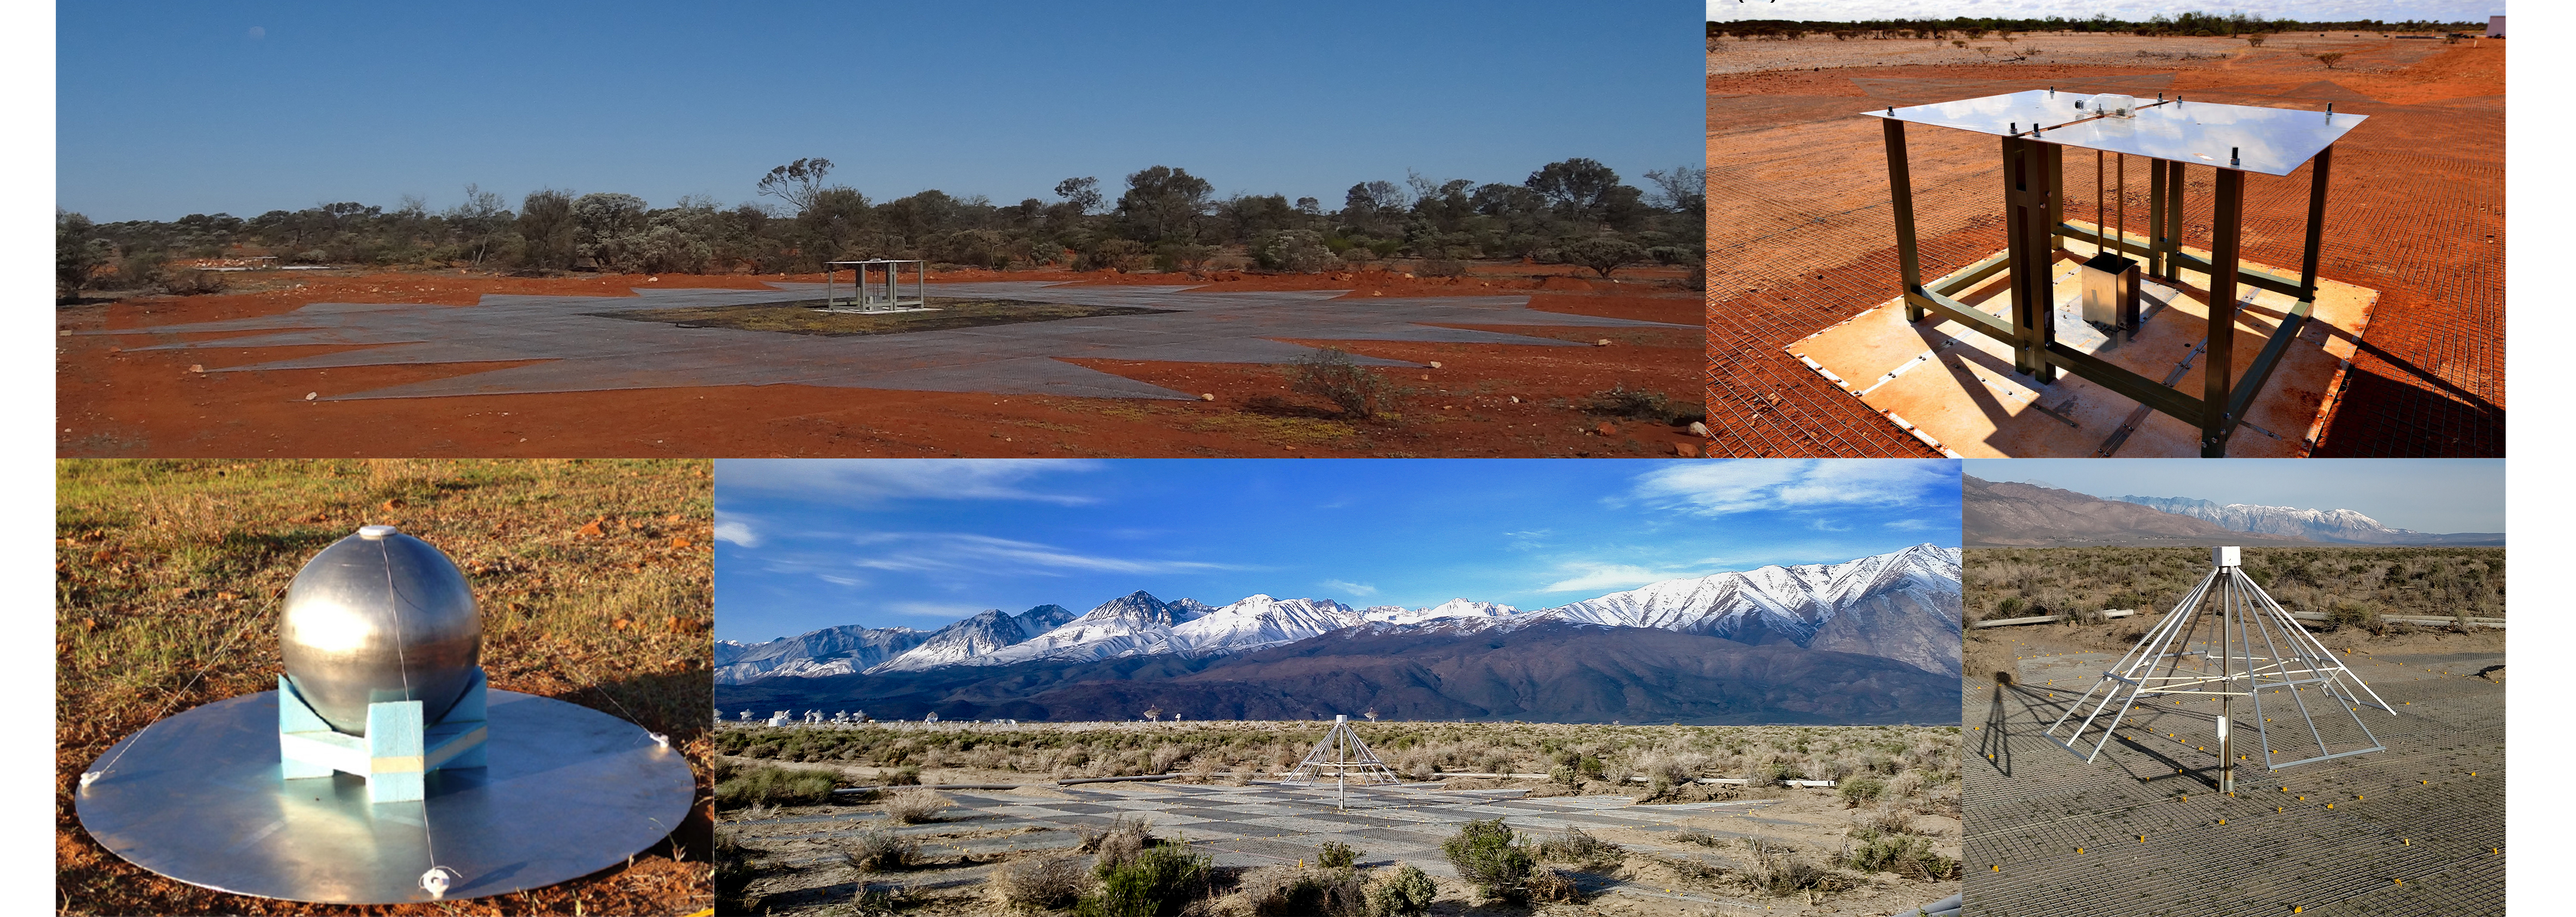
\includegraphics[width=1.05\textwidth]{Greenhill_Subrahmanyan/EDGES_SARAS_LEDA_figure_19sep20.jpg}
\end{center}
\caption{(top left) EDGES antenna and serrated 30~m $\times$ 30~m ground screen.  (top right) Closeup of the EDGES single polarization dipole comprising two rectilinear metal sheets.  (bottom right) Closeup of the LEDA dual polarization pyramidal dipole.  (bottom center) LEDA antenna and serrated 20~m $\times$ 20~m ground screen implemented in 2019. (bottom left) SARAS-2 antenna comprising a spherical element atop a 0.87~m diameter disc.  The maximum gains for EDGES and LEDA antennas are toward zenith.  In contrast, the maximum for SARAS-2 traces a ring on the sky at $30^\circ$ elevation, centered on zenith, where there is a null.}
\end{figure}

\section{Radiometer Basics}

Karl Jansky discovered that any sensor of electromagnetic fields placed beneath open sky samples at its terminals ``cosmic radio noise''\footnote{The term ``noise'' is commonly used because radio frequency (RF) radiation from atomic processes in the cosmos, the ionosphere and troposphere (lightning), and terrestrial thermal sources are spatially and temporally incoherent.  The fields are generally described statistically as Gaussian random variables of zero mean, following from the Central Limit Theorem.}  \cite{jansky33}.  A typical channelized radiometer comprises an antenna, an amplifying receiver that includes a band-limiting filter, a digitizer, and a spectrometer.  The filter defines the measurement bandwidth.   The digitizer samples data at a rate of at least twice the bandwidth.  The spectrometer instantiates Fourier techniques to transform time-series into spectra.\footnote{The theory and implementation of digital spectrometers may be found in \cite{TMS17} and references therein.}  For an Earth-bound antenna, received RF power will include contributions from the cosmos, the ground proximate to the antenna,  self-generated noise from the electronics, and artificial terrestrial interference.  For scale, we note that an antenna with unit gain in equilibrium with a 300\,K blackbody delivers a noise power of {\it O}(1)\,pW over a 100\,MHz band.

\subsection{Antenna}
  
One of the simplest forms of antenna comprises two oppositely directed conductors (a dipole).  Incident waves induce currents in the conductors and a voltage is developed across the inward facing ends (the terminals). The spectrum of power measurable at the terminals corresponds to the incident waves, modified by the frequency-dependent electromagnetic coupling of the antenna and surrounding space (including the ground), antenna efficiency, and transfer function between the terminals and instrumentation downstream.
  
A dipole with wire-like arms each of length one quarter wavelength ($\lambda_0$) will have a sharply peaked resonance and maximum power transfer efficiency at frequency $\nu_0$ in a narrow band $\Delta\nu/\nu_0\ll 1$.  The antenna acts as a transformer from the impedance of free space, $377 \Omega$, on one side to that of transmission lines and RF electronics on the other.  Over a narrow band the impedances of the antenna and RF electronics can be readily matched, and all of the incident power enters the receiver (ignoring resistive losses). 
  
However, the HI signal is inherently broadband, and instrumentation requires at least an octave of bandwidth ($\nu_{\rm high}/\nu_{\rm low}=2$ or $0.66\Bar{\nu}<\nu<1.33\Bar{\nu})$ in order to enable the predicted complex spectral structure due to the 21-cm transition to be distinguished from  smoothly varying foregrounds.  In general, the impedance of a dipole modified to achieve reasonable power transfer efficiency across such broad bandwidths varies considerably in amplitude and phase as a function of frequency.   It can be impossible to match to the RF electronics ``everywhere.''  The consequence is that power is reflected at the antenna-receiver interface and lost. Depending on experiment design, the best that can be achieved with a broadband dipole may be an upper limit on variations in impedance with frequency or an imposed functional form such even in the face of calibration error the variations cannot mimic the science signal.

Broadband dipoles (Figure 1) may be planar with arms comprising 2D shapes (e.g., plates in the case of EDGES), 3D structures comprising planes  (e.g., triangles in the case of LEDA) or more complex structures.  Linear dipoles such as these couple to a single linear polarization mode (with electric field, {\bf E}, oriented along the dipole arms).  Dipoles with spiral and helical arms couple to the circularly polarized mode propagating on axis and jointly to circular and linear modes off axis.  Self-similar planar and conical spirals may have operational bandwidths that exceed an octave and maintain good impedance matching, but other metrics may suffer (e.g., frequency-variable sidelobe structure in gain patterns that generates ``chromaticity'' in antenna response).  Experiments weigh trade-offs differently, typically depending on calibration strategy.

\subsubsection{Ground sensitivity}

Owing to its symmetry, a planar dipole receives radiation incident from the sky and ground equally well.  ``Drooping'' or raising the arms of a linear dipole (e.g., SCI-HI) or projecting a spiral onto a cone--as for the the {\underline B}roadband {\underline I}nstrument for {\underline G}lobal {\underline H}ydrogen {\underline R}eionization {\underline S}ignal--BIGHORNS \cite{sokolowski15}
) are common techniques to break the symmetry, effectively narrowing the field of view and increasing antenna ``directivity.''  However, substantive suppression of coupling to the ground is best achieved by covering it with  a conducting plane.  This ``ground screen'' acts as a reflector.  The antenna senses the sky above {\it and} below, boosting sensitivity for suitable antenna-screen separations (e.g., the direct and reflected paths interfere constructively for $\lambda_0$/4 separation) over some bandwidth. 

Ground screens may be soldered or welded wire mesh, with a minimum conductor spacing or hole size $\ll \lambda_0$, so as to minimize leakage of radiation across the plane.  However, reflection and scattering off the discontinuity represented by the edge of the ground screen creates interference patterns that are functions of the direction and frequency of incident radiation, thereby modulating antenna gain, possibly enough that fluctuations in the received spectrum may be apparent even after calibration.  Adding a random component to the geometry suppresses the effect to a degree.  In telecommunications at high frequencies, fractal-like designs {\it O}($\lambda$) may be etched or milled into a solid metal substrate. However, at low frequencies, sculpting fractals with wire mesh, is impractical.  Instead, implementation of serrated edges has been an effective tool (Figure 1).

%% LJG notes for later.  Confirm adequate treatment of:
%% -Gain pattern characteristics:  achromatic response. 
%% -Electrically small antennas.  Main lobe. 
%% -Antenna impedance characteristics
%% -Tabulation of desirable characeristics that enable radiometry
%%  Editorial comment to consider -- dipoles are good for X.  For 21cm we use them for Y.

% TEXT REMOVED FOR POSSIBLE USE LATER
 %Just as antennas are frequency selective, so also are antenna selective in their direction sensitivity.  I know of no practical antenna that is isotropic.  The relative sensitivity of an antenna across sky directions is referred to as the far-field antenna radiation pattern or beam pattern.  Any antenna is directional and is selective is receiving radiation. A quarter wave dipole antenna is insensitive to radiation incident along its length: after all, radiation incident along that direction would have fields orthogonal to the dipole arms and hence cannot possibly induce currents.  The quarter wave dipole antenna efficiently transduces signals in directions orthogonal to its orientation: quarter wave dipole antennas have toroidal beam patterns; dipole antennas are omni-directional. The larger an antenna is in its electrical size, the more directional is its response to sky radiation.  Antennas with electrical size exceeding unity would naturally have beam patterns that have a main lobe that defines a sky solid angle where sensitivity is maximum, and sidelobes of lower sensitivity.  Electrically small antennas would have a single main lobe without sidelobes.
  
  %Antennas are usually passive systems, hence reciprocal, and may be viewed as radiators or sensors, transforming incident power to signal power at its terminals or transforming power fed at the terminals to free-space radiation.  The antenna as a transformer provides a transformed free-space impedance at its terminals, which is often referred to as antenna impedance. Viewed as a radiator, power fed to the antenna via a transmission line connected to the antenna terminals is only partly available for radiation, because depending on the impedance mis-match between the transmission line and the antenna a part of the power fed to the antenna is reflected back. Of the power available for radiation, a part of the power flows to sky via the main and side lobes of the radiation pattern, a part to ground via what might be considered to be back lobes and a part might be lost as ohmic loss that heats the antenna, if the conducting antenna elements are resistive.  Reflection efficiency of the antenna defines the fractional power available, and radiation efficiency defines what fraction of the available power is radiated into free space.  The antenna views the sky multiplied by the radiation pattern; the weighted average brightness of the sky, with a weighting defined by the radiation pattern, is the sky noise temperature in so far as the antenna is concerned. The radiation efficiency times this temperature is the sky noise temperature component at the antenna terminals, and the reflection efficiency times that terminal noise temperature is the sky noise power propagating down the transmission line.  
  
  %In the context of radiation efficiency, it may also be noted here that if the antenna elements are resistive and there is loss of cosmic signal as ohmic loss in the antenna, not only is there a loss of desired signal but the resistive elements also add their own thermal radio noise to the sky signal. 
  
  %dipole gain patterns are typically broad.  repeating dipoles in parallel giving depth to the structure provide directivity or broad structures, cf. wires  detune but provide coupling over an octave (2x).
 
\subsection{Receiver}

The purpose of an analog receiver is to amplify, over a desired frequency range, the signal coupled to the antenna and passed at it's terminals.  The fluctuating voltage at the terminals propagates along a transmission line to a (typically) modest gain amplifier that boosts signal-to-noise ratios relative to thermal processes in the electronics.  This amplifier too adds noise to the incoming signal, and this is amplified by later stages in the signal path.  There is always a practical trade off between achieving high gain and low noise during amplification, and having the lowest additive noise relative to the sky signal in the first stage amplification is usually paramount, as follows from \cite{friis46}--see also \cite{pozar98} for discussion.  Amplification is most often done in stages, to achieve an aggregate gain sufficient for conversion to a digital signal downstream, without introduction of excessive thermal noise by from particularly high-gain amplifiers. 


\subsubsection{Filtering}

Receivers typically include bandwidth-limiting elements to enhance performance of particular amplifiers or downstream electronics, as for digital processing.  In the former case, filtering is intended to exclude signals that are strong enough to substantively degrade the amplifier linearity, which is susceptible to saturation-like effects, or to create artifacts during amplification where the beating of signals at different frequencies generate products that may be detectable. This is also known as intermodulation (e.g., if broadcast signals above the ``Cosmic Dawn band''  pass through an amplifier, e.g., at 90, 100, and 110 MHz, artifacts may appear in the amplifier output at 10 and 20 MHz).  

For digital processing, filtering serves to suppress the ``aliasing'' of unwanted signals, at frequencies outside the science band, into the band. This occurs when data are sampled at too low rate during digitization.  A digital signal is a sequence of samples.  Sampling with no loss of information requires a rate that is twice the uppermost frequency of interest, as established by the Nyquist-Shannon theorem \cite{TMS17}). Absent application of a sharp low-pass filter corresponding to the top end of the science band, signals at higher frequencies appear to be reflected about the top end and superposed on the science signal.  The unwanted power may be broadcast interference (narrowband) or continuum as from the sky (broadband).

 Common filter topologies are Butterworth, which has a maximally flat, structure-free response, and Chebyshev type 1 and 2, which provides sharper transitions between the passed and rejected intervals but exhibits substantial ripple in one or the other (i.e., the frequency structure to be exiled to where it does the least damage, depending on application).  A third topology, Elliptic, exhibits the same amplitude of structure in the passed and rejected bands, and promises the steepest possible transition from one to the other for a given maximum allowable ripple and magnitude of transition.  Often a combination of filters is used - one to provide excellent rejection but with relatively slower roll-off in response, and others with sharp transitions at the design edges of the passed band.  
   
\subsubsection{Reflection}

Not limited to the antenna-receiver interface, reflection of RF signals occurs at the interfaces between components with different impedances.  A 1\% mismatch in resistive impedance corresponds to a 0.5\% reflection in voltage or 0.003\% in power.  The chain of components along a signal path in a receiver creates instances of multi-path propagation due to numerous fractional reflections.  For well-chosen components, some are negligible, but a complete vector analysis of amplitude and phase is required to understand what frequency structure a receiver may impose in the process of amplifying the input signal.  

In this regard, pairings of filters and amplifiers deserve particular attention.  As noted, filters present frequency structure at their outputs, depending on the selected topology.  They also present frequency structure in reflection at the input. In the case of a low-noise amplifier in the first stage of a receiver, if it is followed by a poorly chosen filter, then it receives back a fraction of its output power but with a potentially complicated frequency-dependent structure imposed.  This propagates upstream through the amplifier (with finite loss, a.k.a. isolation) and reflects off the imperfect antenna-receiver interface and arrives at the amplifier input, added to the cosmic signal and conceivably at detectable levels.

Analysis of multi-path propagation among components applies to additive  thermal noise as well as the amplified sky signal.  Where noise and an attenuated, phase-shifted reflection are co-added during propagation, it develops frequency structure, even though for any given circuit temperature, the noise intrinsically varies slowly and smoothly with frequency.  Because the antenna-receiver interface presents the largest mismatch along the signal path, this is especially important in the case of the first amplifier, from which noise propagates upstream toward the antenna as well as downstream toward later stages of amplification.

A primary engineering formalism describing noise characteristics of linear devices involves a quartet of parameters, one for each frequency:  minimum noise temperature, optimum voltage reflection coefficient (magnitude), the optimum voltage reflection coefficient (phase), and the equivalent noise resistance (referring to the spectral density of noise).  These may be used to estimate the frequency structure impose on noise emanating from amplifiers, as well as the dependence of the amplifier noise temperature on frequency and impedance.  (An amplifier facing a resistive (real) or reactive (imaginary) impedance at its input exhibits different gain and noise temperature.)  Building off \cite{hu04}, \cite{rogers12}  present a simplified formalism for low-frequency systems referred to as ``noise wave'' analysis, which characterizes propagation of noise in terms of correlated and uncorrelated components.  As applied, this works well provided that the reactive component outside the amplifier is sufficiently small. 

\subsection{Digitzer}
  
Analog-to-digital converters (ADC) sample the receiver output at the ``Nyquist rate,'' described above (e.g., 5\,ns for a bandwidth of 100\,MHz).  The number of bits used to represent each sample determines the dynamic range achievable in each spectrum generated by a Fourier transform of every $N$ samples (e.g., for $N=4096$, the frequency resolution, $R$, in the above example is 24.4\,kHz).   The number of bits per sample must be sufficient to represent the range of sky brightness integrated over the antenna gain pattern and prescribed bandwidth. In particular for a sky with a steep spectral index and/or antenna with steep change of gain with frequency, there must be enough bits to represent power at both the highest and lowest frequencies.  At present, transport of an aggregate data rate of {\it O}(2)\,Gbit s$^{-1}$ can be readily achieved, corresponding to 10-bits per sample and a $2^{10}$:1 dynamic range for voltage and $2^{20}$:1 for power.
ADC hardware providing 8 to 16 bits at sample ranges {\it O}(100)\,MHz is readily available.  However, the minimum acceptable bit depth for a given site often depends on the presence and characteristics of interference.  Where peak band-averaged power due to continuous or impulsive interference exceeds that of the sky, representing both without saturation demands greater bit depth in sampling.  Additional considerations arise in  the uniformity of steps during quantization of analog data, linearity over the full analog range, and calibration accuracy where sampling may be parallelized over multiple samplers (a.k.a. interleaving).
 
\section{Challenges Facing Experiments}

\subsection{Antenna Radiation Efficiency}

If an antenna is lossless and has no resistive elements, then when viewed as if it were a transmitting all of the power fed to the antenna, and not reflected back along the transmission line at the antenna terminals, will emerge as radiation.  However, for an antenna placed on bare ground, part of the radiated power may be absorbed.  Low-frequency electromagnetic waves penetrate soil to substantial depths: several meters for dry soil. For antennas that are placed on an infinite conducting ground screen, all of the radiated power goes to sky either directly or on reflection off the ground screen. Passive reciprocal antennas may be viewed conversely as receivers where the loss to resistive elements of the antenna and the loss to the ground both reduce antenna radiation efficiency while adding thermal noise.
   
However, ground loss has a role in mechanisms that create two additional challenges where redress may be more difficult. First, the additive component of ground emission has a complex imprint of the antenna radiation efficiency, making it difficult to separate from zero-mode 21-cm signals unless the antenna is designed so that the radiation efficiency itself has characteristics orthogonal to expectations for zero-mode signals.  Second, the loss depends on ground characteristics, specifically conductivity and dielectric constant, which depend on soil characteristics and moisture content and are functions of depth and time. A sudden change in dielectric constant or conductivity at depth created an impedance discontinuity, as does intrusion of bedrock into the strata.  Such a discontinuity drives multi-path propagation among ground layers and instrumentation above--e.g., see \cite{bradley19}.  Mapping and tracking the RF characteristics of the ground can require extensive additional dedicated instrumentation, such as a network of dielectric impedance reflectometers, and tools to make use of the data are relatively crude at present.
   
Antenna radiation efficiency is also influenced by the environment of the antenna, not only the ground beneath but also feature above, such as shrubs and man-made structures at distances up to several wavelengths.  Conducting cables that supply power to the radiometer and conduct signals to receivers located some distance away may also influence the efficiency.  In measurements of the reflection efficiency as a transmitting antenna, power transmitted by the antenna reflect and scatter off trees and structures in the environment and return to the antenna, as in a radar. Thus measurements of $\Gamma$ sample the environment as well as the antenna.  Conversely, these environmental features will influence the receipt of cosmic radiation in reverse.  Scattering off these objects may generate spectral structure that is an imprint of the environment.  Thus, it is essential to have a clear space above ground and homogeneous if not also dry soil below.

\subsection{Antenna Transfer Efficiency}
   
   The antenna transfer or reflection efficiency, $(1-\Gamma^2)$, which is related to the voltage reflection coefficient $\Gamma$ at the antenna terminals, determines what fraction of cosmic noise received by the antenna propagates into the receiver chain.  In this consideration, it is the impedance of the antenna at its terminals, which is effectively the free space impedance transformed by the antenna to its terminals, as compared to the impedance of the first low noise amplifier encountered by the cosmic noise as transformed by the interconnecting transmission line to the antenna terminals, that decides the reflection coefficient $\Gamma$.  
   
   A design goal for zero-mode 21 cm is an antenna that has high reflection efficiency over the full observing band.  However, since the foreground Galactic sky has a brightness temperature that is significantly greater than the noise temperatures of modern low noise amplifiers operating in the 10-200 MHz band, it is sufficient that the total efficiency of the antenna provide an antenna temperature that well exceeds the receiver noise.  In that case, the system temperature and hence the measurement noise for any integration time would be independent of the receiver noise and improving the total efficiency would not improve detection sensitivity or reduce the required observing time.
   
   What is probably of greater importance is that the reflection efficiency be a smooth function of low order so that the product of the relatively bright foreground sky with the reflection efficiency, to give the dominant unwanted component of the observed spectrum, does not confuse the desired zero-mode 21 cm signal, and is separable from the 21-cm signal.  If the antenna structure is electrically long, as would be the case, for example, in frequency independent spiral antennas with large structural bandwidth, the reflection efficiency would have fine structure in frequency.  Therefore, from the viewpoint of designing the antenna element to have reflection efficiency that is exclusively of low order, it is advantageous to have electrically small antennas.
   
   If the antenna does not have resistive elements, and the radiation efficiency is unity, then a measurement of the antenna reflection efficiency $\Gamma$ would be a useful method for correcting the data for antenna efficiency and translating the measured spectrum to a sky spectrum. In this case, it is desirable and useful to provide a switch at the antenna terminals, which might allow a 1-port network analyser to access the antenna terminals and make an accurate measurement of $\Gamma$.  This is best done at the observing site, where the antenna environment is the same as for the zero-mode observing.  Deriving the reflection efficiency and total efficiency requires also a measurement of $\Gamma$ for the low-noise amplifier, but that may be done in the laboratory provided that the amplifier temperature and operating conditions are the same.

\subsection{Gain Pattern}

A critical challenge in antenna design is suppression of ``mode coupling.'' This arises when an antenna gain pattern is chromatic, i.e., for each direction, gain varies with frequency. \footnote{We note in passing that there is no general, compact, quantitative definition of chromaticity.}   Even for a sky with a constant spectral index, the consequence of chromatic response is potentially complex frequency structure everywhere on the sky.  

Mode-coupling can be a fundamental hurdle to detection of the 21-cm signal with any given antenna.  The most certain means to suppress it is to adopt antennas that are achromatic, i.e., frequency-independent in gain in all directions.  Chromaticity may not be easily quantified, but spectra being limited by statistical noise rather than undulations in the spectral baseline can be an effective figure of merit.  Servicing this, spectra simulated using calculated gain patterns and sky models may be used in tuning antenna designs to achieve a required level of a-chromaticity.

\subsubsection{Measurement and Simulation}

High-accuracy direct calibration of gain patterns {\it in situ} (thereby taking into account all details of coupling to the ground, structures, ground screens, etc) is an unsolved problem.  There are no suitable standard antennas in communications engineering.  Lofting transmitters on drones has been developed \cite{jacobs17}, but cancellation of systemtics intrinsic to this scheme (e.g., multi-path and uncertainty in the gain pattern of the transmitting antenna) has not been demonstrated and confirmed.  The most widely employed alternative is numerical simulation.

Arguably, most available electromagnetic simulation packages are not capable of providing solutions with the precision necessary to quantify antenna response, though cross-referencing of results enables assessment of systematics stemming from the various simulation techniques applied.  Exacerbating the above difficulty is the need to include in simulations coupling to stocastic elements in the surroundings (vegetation), soil chemistry, and time-variable changes in water content. Antennas also couple to strata below ground with complex permittivities (i.e., non-zero conductivity) and infrasructure such as trenched cables.  In general the design path necessarily requires iteration to achieve exacting performance tolerances, and cross-referencing results obtained with different packages.   

\subsection{Cosmic Foregrounds}

At millimeter wavelengths where the CMB peaks the sky is dominated by the CMB. Galactic emission and the extragalactic background are sub-dominant.  At frequencies relevant to the 21-cm transition at high $z$, the radio sky is qualitatively different, dominated by synchrotron emission from the Galactic plane, which extends to considerable latitudes, and diffuse off-plane components.  As well, in neither case is the structure readily modeled in angle or frequency, not least because position-resolved spectra of the sky at these low frequencies are known with accuracies of only {\it O}(10\%).  Moreover, there are no known fiducial tracers that may be used to establish external constraints.

The peak amplitude of the cosmic 21-cm signal is expected to be a few tens to a few hundred mK, and the foreground is expected to between a few hundred to a few thousand Kelvin brightness temperature.  This requires a dynamic range of at least $10^4$, clean signal detection requires aiming for dynamic range of $10^5$.  Because the algorithms for components separation, which depend on orthogonality between the zero-mode 21-cm signal and other unwanted additives and foreground, are usually limited and the models for the unwanted components would subsume a significant part of the 21-cm signal; therefore, the typical design goal for the 21-cm radiometers is to achieve an artifact-free spectrum of {\it O}(1)\,mK sensitivity, about $10^6$ below the dominant foreground.

\subsection{Ionosphere}

The ionosphere has time varying electron densities that is commonly characterized by the total electron content (TEC) along any line of sight.  The ionosphere modifies spectra of background sources in several ways.  It refracts rays, so that sources appear at higher elevations \cite{vedantham14}.  The ionosphere also both absorbs the background and adds emission from populations of hot electrons \cite{rogers15}. These effects of the ionosphere are strongly wavelength dependent and are anticipated to predominantly modify radiation at $\nu\lesssim 100$\,MHz.

In general, the accuracy and spacing of TEC measurements is as yet inadequate to support time-varying correction of measured sky spectra.  TEC data are primarily of use in deciding the relative severity of ionospheric conditions and the order of magnitude of distortions to be anticipated in spectra--a coarse weather report.  Consequently, analyses of radiometry data  must include model nuisance parameters that describe ionosphere effects, requiring marginalization in order to extract the zero-mode signal from data.  

\subsection{Polarization}

Galactic and extragalactic foregrounds comprise sources often with significant fractional  linear polarization.  The detected foreground spectrum will be polarisation dependent.  Complications arise due to Faraday rotation of differing degrees.  The effect is frequency  dependent, and for a linearly polarized source, the source intensity received by any single polarization will be frequency dependent.  Hence, Faraday rotation results in spectral structure that may potentially confuse attempts to detect zero-mode 21-cm spectral structure. For this reason, it is desirable and a design goal for zero-mode radiometers to be dual polarised pair of radiometers, with full polarisation calibration that allows derivation of the Stokes I component on the sky.


\subsection{Interference}

Virtually all frequencies at which a zero-mode signal corresponding to the EOR or CD could appear are allocated to terrestrial and space communications. Transmitters at these frequencies exist in most parts of the world, and propagation paths may be line of sight, reflected (e.g., off meteor trails and aircraft), or bent by diffraction around obstacles. Extremely remote sites exist where interference due to long-range propagation is rare \cite{voytek14,philip19}, but apart from these unusual cases, low-frequency radiometry data is corrupted intermittently, raising the possibility of weak interference contributing weak artifacts in spectra.  These may be narrow band (e.g., FM transmission) or broadband (e.g., digital television, where each channel allocation is several MHz wide).  They may be recognizable as discrete spectral features or solely by deviations from Gaussian statistics in time-series.


\section{Pr\'ecis of Design Requirements}


\begin{itemize}
    \item[1.]
    {\bf Radiometer bandwidth}: an octave or more, to enable separation of smooth-spectrum foregrounds and the distinctly not smooth 21-cm spectral signature.
    
    \item[2.]
    {\bf Antenna gain pattern {\it in situ}}: maximally smooth in angle and frequency with minimum chromaticity, and characterization from direct measurement or simulation if necessary.
    
    \item[3.]
    {\bf Ground screen}: large enough to isolate the radiometer from propagation in ground strata and buried infrastructure); sufficient geometric irregularity along the edges so as to suppress coherent patterns in scattering of incident radiation toward the antenna. 
    
    \item[4.]
    {\bf Antenna polarization}: dual polarization to enable construction of Stokes I and cancel artifacts that can arise from Faraday rotation of foreground emission.
    
    \item[5.]
    {\bf Site}:  a radiometry site with a clear horizon out to several wavelengths, and related to item no. 3,k homogeneous dry strata below.

\end{itemize}



   
   
%\subsection{Reflections within the Signal Path}

 % Impedance discontinuities in the receiver path cause internal reflections of the system noise, which includes the cosmic noise component and also the receiver noise.  Reflections of wideband noise over a physical length $l$ result in interference that cause spectral structure with frequency scale $v/2l$, where v is the propagation speed of electromagnetic waves in the physical medium.  For example, internal reflection within a cable of length 2 metres between the antenna and low-noise amplifier, with velocity factor 0.7, will result in spectral ripples with period 52.5 MHz. These structures would be a modulation of the receiver gain, and hence calibrated out, if the calibration includes these sections in their entirety.  However, if the receiver calibration is internal, then reflections from the antenna terminal and also reflections of receiver noise from environment are omitted from the calibration.  Ideally, receiver gain calibration using celestial sources, such as the passage of the Galactic plane across the radiometer beam, would best calibrate the signal path.  In any case, it is desirable that the signal path have isolators that prevent back flow of signal path components to the antenna.  Improved isolation also comes from use of amplifiers in which the forward gain is substantially greater than the reverse isolation, so that the net loss on propagation back and forth is substantial.
  
  
%\subsection{Analog to digital conversion}
 
% A key component in the signal processing in a zero-mode 21-cm radiometer is the conversion from continuous to discrete data.  Random and systematic errors in the representation of the analog signal leads to performance limitations.  An important design consideration is the number of bits in the analog to digital converter.  Larger effective number of bits is essential for greater spurious free dynamic range.  A design goal of $10^6$ for dynamic range requires 10 effective bits, which implies analog to digital converters of 12 bits or greater.  The quality in the transfer function of the converter is also required to be accurate so that the spurious free dynamic range is $10^6$.
 
%\subsection{Radio Frequency Interference (RFI)}
  
%  Radio frequency interference (RFI), if present at the observing site, would naturally require improved performance of the radiometer to avoid spurious spectral structure that might confuse the zero-mode signal.  In good sites, it is expected that the total power in RFI would be well below the total band power from cosmic noise.  This is facilitated by adopting small antenna designs that have low gain, low effective collecting area, so that the cosmic noise is received without compromise but response to RFI is reduced. 
 
% Presence of radio frequency interference may drive the design to lower the power in the cosmic noise going to the analog to digital converter, so that the signal is not clipped in the sampling, which would lead to non-linear products spread across the band.  Lowering the power in the cosmic noise, to provide greater headroom for the RFI components when they might occur, reduces the effective number of bits operating on the cosmic noise, thus requiring greater performance of the analog to digital converter.
   

%\subsection{Receiver Design}

%The receiver modifies the cosmic radio spectrum in its bandpass, and adds receiver noise; these require bandpass calibration and correction of the measurement data for additives.  Most receiver designs adopt methods for cancellation of additives, via switching schemes.  However, there may be additives that suffer multi-path propagation that includes reflection off the antenna impedance, which may not be canceled.  In such cases, receiver designs often incorporate isolators and also minimise physical lengths of multi-path propagation, so that the unsubtracted additives are restricted to be of low order and hence largely orthogonal to the 21-cm signals.


\section{Outside the Box Architectures}

\subsection{Single-element Sensor  Radiometer}
  
  The simplest form of a radio telescope that would be appropriate for detecting the zero-mode 21-cm signal is a single elemental wideband antenna followed by a spectrometer.  Such a radiometer would ideally have a frequency-independent antenna, a self-calibratable receiver that corrects for the bandpass, and switching schemes to cancel internal additives including receiver noise.
  
  The considerations that drive the design of such a radiometer have been discussed above.  Limitations and design challenges to the performance of such a single-element spectral radiometer are manifold.  Therefore, there have been new concepts and design attempts to develop alternate schemes or configurations that might avoid some of the potential show stoppers.
  
\subsection{Outriggers to Fourier Synthesis Telescopes}
  
  A key challenge in zero-mode 21-cm radiometers is knowing the antenna beam pattern, its chromaticity, and the bandpass of the antenna element.  Antenna measurements at long wavelengths are exceedingly difficult because of the parasitic effects of environment and the ground, which influence both the device under test and also the test and measurement antenna.  Switched calibration, using broad band noise sources, may serve to calibrate the bandpass of the receiver chain; however, this leave the antenna bandpass, radiation efficiency, uncalibrated.  This leads to a situation where the antenna characteristics may have to be derived from electromagnetic simulations, which may not have the accuracy needed for correction of the measurement data.
  
  A solution to these issues is to deploy the single-element sensor based radiometer as an outrigger to an array of antennas, which operate in Fourier synthesis interferometer mode.  The radiometer antenna and receiver chain then form another element of the array, which together observe the sky sources within the antenna primary beams.  The measured spectral visibilities are then used to solve simultaneously for the sky model and also the instrument parameters, which include the bandpass and beam shape of the outrigger antenna. If all array elements are dual polarised, then full Stokes calibration is also possible, providing polarisation calibration solutions as well for the outrigger antenna.
  
\subsection{Interferometric Methods}
  
  It is not often appreciated that interferometers are not totally blind to the zero-mode in the sky temperature distribution.  If the sky were uniformly bright, then the electromagnetic fields at two points in space separated by less than a wavelength will show mutual coherence, which may be measured by an interferometer.  A pair of half-wave dipoles placed adjacent to each other, in line, will respond to the zero-mode of the sky temperature distribution.  If placed parallel to each other the interferometer response will contain the zero mode, and the response in this case will be greater.  The interferometers may be thought of as sampling the zero-mode in the direction in which the projected spacing between the elements in zero.  Of course, if the spacing between the dipoles increases, the response falls off progressively.
  
  The coupling of the interferometer response to the zero-mode signal depends on the mutual coupling between the aperture fields in the pair of antennas.  This is relatively high for closely spaced elemental antennas; however, a pair of aperture antennas placed adjacent to each other would have very little response to the zero-mode if their aperture illuminations have little overlap.
  
  Interferometers have the advantage that when they deploy a pair of sensors of the electromagnetic field at two separated locations in space, and measure the mutual coherence in the fields by cross correlating the received and amplified voltage waveforms, they are insensitive to the additive receiver noise in the two arms, which are uncorrelated.  
  
  Thus interferometer measurements are blind to internal receiver additives, thus scoring over single element radiometers on this count.
  
\subsection{Zero-spacing Interferometer}
  
  If a pair of wideband antennas are placed adjacent to each other, with mutual coupling between the antennas, then the interferometer response includes the zero-mode signal.  This response may be enhanced by placing a vertical beam splitter in between the antennas, so that incident field from any side propagates to the antenna on the far side through the screen and to the near side in a direct path and also after reflection off the screen.  If the beam splitter is reactive, and lossless, then the response to zero-mode on the two sides of the screen cancel.  However, if the beam splitter is resistive, then the interferometer responses add with the same sign.  Optimally, it can be shown that the sensitivity is a maximum if the beam splitter has a sheet resistance equal to the impedance of free space.  
  
  Interferometers made from elemental antennas placed in a close packed configuration will have a telescope filter function, which defines the interferometer response to zero-mode 21-cm signals, that is highly frequency dependent and challenging to calibrate.  The advantage of the zero-spacing interferometer made from frequency independent antennas is that the telescope filter function in this case is flat, at least over the frequency range in which the resistive screen is frequency independent.  
  

\subsection{Lunar Occultation}
  
  An alternate and interesting approach to detection of the zero-mode 21-cm signal is via Fourier synthesis imaging of the Moon.  The brightness measured towards the Moon, over frequency, would be a difference between the Moon brightness and the mean brightness of the radio sky.  Thus if the Moon were assumed to be of flat spectrum, or if the temperature spectrum of the Moon were known, then the differential measurement may be used to infer the zero-mode 21-cm signal.
  
  The measurement is not without difficulties.  Firstly, it is not clear that the temperature spectrum of the Moon is flat of even smooth; the lunar regolith may have structure and layered in depth, which would give spectral structure in the emission brightness.  Additionally, the Moon is reflective and hence the brightness of the Moon has a component that is a reflection of the radio sky. Finally, the synthetic beam of the Fourier synthesis telescope will have sidelobes that are chromatic; thus mode coupling will induce spectral structure whose removal from the data will be limited by the depth of deconvolution. 
    





%=============================================

\bibliographystyle{plain}
\bibliography{Greenhill_Subrahmanyan/References}
%\bibliography{./references}

%=============================================



